\documentclass[11pt,a4paper]{article}
\usepackage[left=2.2cm,right=2.2cm,top=2cm,bottom=2cm]{geometry}
\usepackage[T1]{fontenc}
\usepackage{charter}
\usepackage{amsmath}
\usepackage{graphicx,booktabs,tabularx,enumitem,xcolor,float}
\usepackage{tikz}
\usetikzlibrary{positioning,arrows.meta,fit,backgrounds}
\usepackage[hidelinks]{hyperref}
\setlist{itemsep=1pt,topsep=2pt}
\newcolumntype{Y}{>{\raggedright\arraybackslash}X}
\newcommand{\fillin}[1]{\textcolor{red}{[#1]}}
\input{../final_report/team.tex}

\begin{document}

% ---------------- title page ----------------
\begin{titlepage}
\centering

\includegraphics[width=3.2cm]{iitp_logo.png}\\[0.6cm]
{\Large\bfseries Indian Institute of Technology Patna}\\[2pt]
{\large Department of Computer Science and Engineering}\\[1.4cm]
{\large CS5103 Computing Lab --- Agentic AI Assignment}\\[0.5cm]
{\LARGE\bfseries AutoGrader: A Rule-Driven Evaluator\\[3pt] Agent for C Programs}\\[0.5cm]
{\large Phase 1 Project Report (agentic01)}\\[2pt]
{Plan, work distribution, progress and timeline}\\[1.4cm]
{\large Submitted by}\\[0.4cm]
\begin{tabular}{ll}
\toprule
\textbf{Name} & \textbf{Roll number}\\
\midrule
\memA & \rollA\\
\memB & \rollB\\
\memC & \rollC\\
\memD & \rollD\\
\bottomrule
\end{tabular}\\[1.4cm]
{\large Instructor: Prof.\ Arijit Mondal}
\vfill
{\large 22 October 2026}
\end{titlepage}

% ---------------- 1 ----------------
\section{Objective}
An agent that takes a student's C submission and an instructor's rules file, runs the program
safely, checks it against every metric in the rules, and returns one reproducible grade with
feedback: the failing input, the expected output beside the actual one, and the reason.
The contract we design around: \emph{same submission + same rules $\Rightarrow$ same grade}.

% ---------------- 2 ----------------
\section{Proposed architecture}

\begin{figure}[H]
\centering
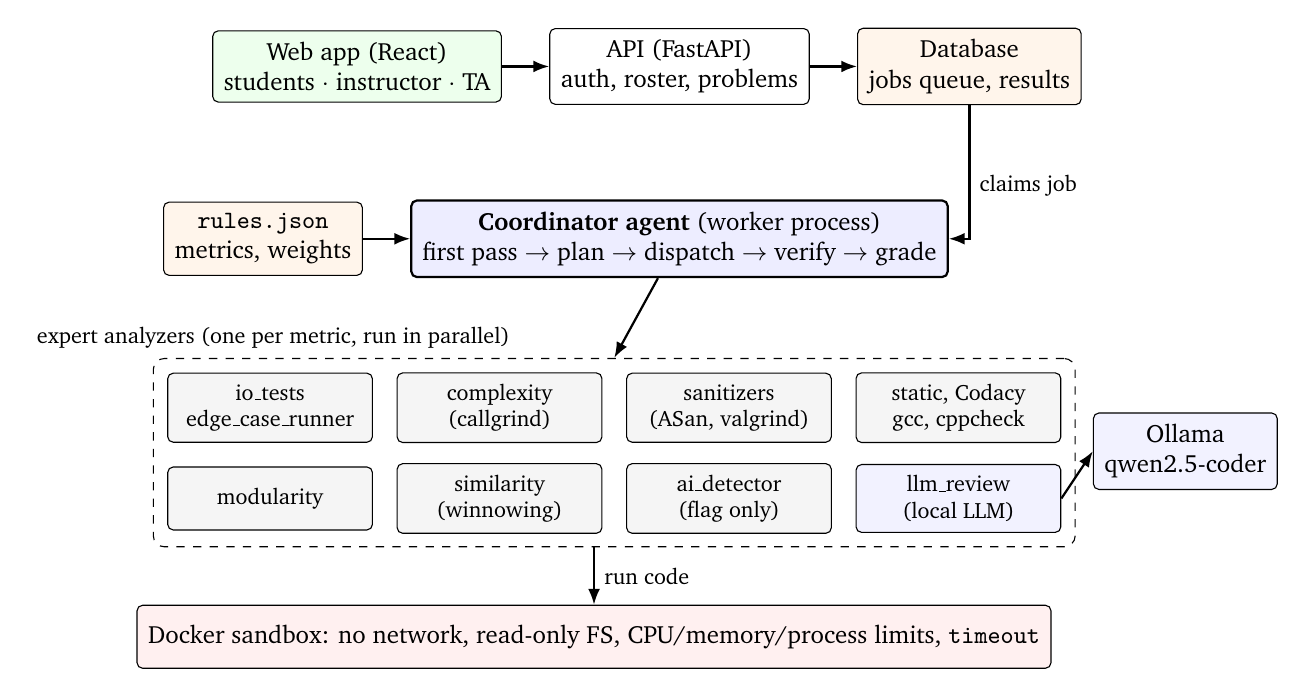
\begin{tikzpicture}[
  font=\small, node distance=4mm and 6mm,
  box/.style={draw, rounded corners=2pt, align=center, inner sep=4pt, minimum height=8mm},
  agent/.style={box, fill=blue!7, thick},
  tool/.style={box, fill=gray!8, font=\footnotesize, minimum width=26mm},
  store/.style={box, fill=orange!8},
  arr/.style={-{Latex[length=2mm]}, thick}]

\node[box, fill=green!7] (ui) {Web app (React)\\ students $\cdot$ instructor $\cdot$ TA};
\node[box, right=of ui] (api) {API (FastAPI)\\ auth, roster, problems};
\node[store, right=of api] (db) {Database\\ jobs queue, results};
\node[agent, below=12mm of api, minimum width=60mm] (coord)
  {\textbf{Coordinator agent} (worker process)\\
   first pass $\rightarrow$ plan $\rightarrow$ dispatch $\rightarrow$ verify $\rightarrow$ grade};
\node[store, left=6mm of coord] (rules) {\texttt{rules.json}\\ metrics, weights};

\node[tool, below=12mm of coord, xshift=-52mm] (t1) {io\_tests\\ edge\_case\_runner};
\node[tool, right=3mm of t1] (t2) {complexity\\ (callgrind)};
\node[tool, right=3mm of t2] (t3) {sanitizers\\ (ASan, valgrind)};
\node[tool, right=3mm of t3] (t4) {static, Codacy\\ gcc, cppcheck};
\node[tool, below=3mm of t1] (t5) {modularity};
\node[tool, right=3mm of t5] (t6) {similarity\\ (winnowing)};
\node[tool, right=3mm of t6] (t7) {ai\_detector\\ (flag only)};
\node[tool, right=3mm of t7, fill=blue!5] (t8) {llm\_review\\ (local LLM)};

\node[box, below=9mm of t6, xshift=12mm, fill=red!6] (sb)
  {Docker sandbox: no network, read-only FS, CPU/memory/process limits, \texttt{timeout}};
\node[box, right=4mm of t8, yshift=6mm, fill=blue!5] (llm) {Ollama\\ qwen2.5-coder};

\begin{scope}[on background layer]
\node[draw, dashed, rounded corners, fit=(t1)(t4)(t5)(t8), inner sep=5pt, label={[font=\footnotesize]above left:{expert analyzers (one per metric, run in parallel)}}] (ex) {};
\end{scope}

\draw[arr] (ui) -- (api);
\draw[arr] (api) -- (db);
\draw[arr] (db) |- (coord.east) node[pos=0.3, right, font=\footnotesize] {claims job};
\draw[arr] (rules) -- (coord);
\draw[arr] (coord) -- (ex.north) ;
\draw[arr] (ex.south -| sb.north) -- (sb.north) node[midway, right, font=\footnotesize] {run code};
\draw[arr] (t8.east) -- (llm.west);
\end{tikzpicture}
\caption{The API never runs student code. A separate worker runs the coordinator agent, which
dispatches one analyzer per metric. Analyzers that execute code use the sandbox, and only
\texttt{llm\_review} (plus optional feedback text) calls the local model.}
\end{figure}

\paragraph{How one submission is graded.}
\begin{enumerate}
  \item \textbf{First pass.} Compile with \texttt{-Wall -Wextra}, run the sample input once, and check for \texttt{main}, input and output.
  \item \textbf{Plan.} If the program does not compile or hangs, the run-based analyzers are skipped and the quality metrics score 0; the rest still run.
  \item \textbf{Dispatch.} The analyzers named in \texttt{rules.json} run in parallel, each in its own sandbox.
  \item \textbf{Verify.} Inputs suggested by the LLM count only if running them against \texttt{reference.c} confirms a failure.
  \item \textbf{Grade.} $\text{grade}=\sum_i \text{score}_i\times\text{weight}_i\times 100$, computed in code. The LLM never decides correctness.
\end{enumerate}

\paragraph{Design decisions.}
\begin{itemize}
  \item \textbf{Execution decides, the LLM advises.} A local code model (no fine-tuning; temperature 0, fixed seed, cached replies) reviews readability, and its prompt includes verified findings from Codacy, cppcheck and gcc. Tests and sanitizers decide correctness.
  \item \textbf{Rules outside the code.} Adding or re-weighting a metric is a JSON edit. The hash of the rules is stored with every grade.
  \item \textbf{Reproducibility.} Seeded test generation, instruction counts (not wall-clock time), cached LLM replies, and hashes of the submission, rules and tests in every report.
  \item \textbf{Originality.} MOSS-style winnowing against classmates, a web corpus and an LLM-generated corpus. Copy and AI signals are flags for the instructor to review; students only see confirmed ones.
\end{itemize}

% ---------------- 3 ----------------
\section{Metrics (example rule set)}
\begin{tabularx}{\textwidth}{@{}llYr@{}}
\toprule
\textbf{Metric} & \textbf{Analyzer} & \textbf{Method} & \textbf{Weight}\\
\midrule
correctness & io\_tests & hidden tests, output compared after normalisation & 0.20\\
syntax & compiler\_warnings & gcc \texttt{-Wall -Wextra}, penalty per warning & 0.10\\
structure & static\_analysis & cyclomatic complexity, function length, cppcheck & 0.10\\
modularity & function\_split & call graph from \texttt{main} & 0.10\\
logical & edge\_case\_runner & named edge cases + 100 seeded random inputs vs.\ reference, counter-examples shrunk & 0.10\\
complexity & complexity\_estimator & valgrind instruction counts fitted to $O(1)\dots O(n^3)$ & 0.10\\
memory\_safety & sanitizer\_run & AddressSanitizer, UBSan, valgrind leak check & 0.10\\
readability & llm\_review & rubric prompt to local model, injection guard & 0.10\\
originality & similarity\_flag & winnowing fingerprints, threshold 0.85 & 0.10\\
\bottomrule
\end{tabularx}

\smallskip
We also plan two optional metrics: \texttt{codacy\_review} (Codacy static analysis) and \texttt{ai\_detector} (flag only, weight 0).

% ---------------- 4 ----------------
\section{Distribution of work}
\begin{tabularx}{\textwidth}{@{}lY@{}}
\toprule
\textbf{Member} & \textbf{Responsibility}\\
\midrule
\memA & Coordinator agent, rules format, sandbox, job queue, integration and testing\\
\memB & Execution analyzers: I/O tests, edge cases and counter-examples, complexity estimation\\
\memC & Code-quality analyzers: compiler warnings, static analysis, modularity, sanitizers, Codacy\\
\memD & LLM review, originality and AI-origin detection, choice of local model; web interface\\
\bottomrule
\end{tabularx}

% ---------------- 5 ----------------
\section{Progress so far}
In this first phase we studied the problem, surveyed the tools, and fixed the architecture above.
\begin{itemize}
  \item \textbf{Requirement study.} We read the assignment and mapped every requirement to a component: sandboxed execution, external rules, one analyzer per metric, failing input with expected output, copy/LLM flagging, usefulness and limitations.
  \item \textbf{Sandboxing.} We compared running programs directly (with \texttt{timeout}/\texttt{prlimit}) against Docker containers and chose Docker. It gives no network, a read-only file system and process and memory caps, and it behaves the same on Windows and on the lab's Linux machines.
  \item \textbf{Analysis tools.} We tried gcc warnings, cppcheck, AddressSanitizer, UBSan and valgrind (memcheck for leaks, callgrind for instruction counts) on small buggy C programs and decided which metric each one serves.
  \item \textbf{LLM.} We studied whether the model needs fine-tuning. A pre-trained code model with a rubric prompt, temperature 0 and a fixed seed is enough for readability feedback, as long as correctness is decided by execution. We picked Ollama with a local model (qwen2.5-coder) because the course requires local models.
  \item \textbf{Originality.} We studied MOSS-style winnowing for copy detection and decided on three corpora: classmates, known web solutions and LLM-generated solutions.
  \item \textbf{Technology stack.} Python with FastAPI for the agent and API, a separate worker process for grading, SQLite for storage, and React for the web interface.
  \item \textbf{Setup.} We prepared the development environment (Python, Docker image with gcc, valgrind and cppcheck, Ollama) and the first sample problem with its rules file and test cases.
\end{itemize}

% ---------------- 6 ----------------
\section{Plan and timeline}
\begin{tabularx}{\textwidth}{@{}lY@{}}
\toprule
\textbf{Week} & \textbf{Work}\\
\midrule
10--16 Oct & Requirement study and research on tools \emph{(done)}\\
17--22 Oct & Architecture, rules format, technology choice, environment setup \emph{(done)}\\
23--29 Oct & Implement the coordinator, the sandbox and all analyzers; first end-to-end grade on the sample problems\\
30 Oct -- 5 Nov & Web interface, testing (including malicious programs), final report, GitHub repository, video\\
\bottomrule
\end{tabularx}

% ---------------- 7 ----------------
\section{Expected usefulness and limitations}
\textbf{Useful for:} grading a whole lab unattended with explainable per-metric marks;
showing each student the exact input that breaks their program; narrowing plagiarism review
to the flagged pairs; screening coding-test submissions.

\noindent\textbf{Limitations we expect:}
\begin{itemize}
  \item Tests cannot prove correctness. A bug that no hidden test or generated edge case triggers would still get full marks.
  \item An LLM's readability score can change with the model or the hardware, so replies must be cached to keep grades reproducible.
  \item Similarity on very short programs is unreliable, because every correct two-line answer looks alike.
  \item An AI-origin signal can flag a careful human writer, so it should never change the grade by itself.
\end{itemize}

\end{document}
